\section{Versuchsdurchführung}
\subsection{Teil I: Pockels-Effekt}
\subsubsection{Bestimmung der Halbwellenspannung mit einer Sägezahnspannung}
Um eine grobe Abschätzung der Halbwellenspannung zu bekommen,
wird im ersten Versuchsteil an die Pockelszelle das Sägezahnsignal angelegt.
Gleichzeitig wird mit dem Oszilloskop das Spannungssignal nach dem Verstärker der Photodiode gemessen.
Durch Drehen des Analysators wird dieses Signal so eingestellt,
dass die Amplitude maximal ist, aber kein \emph{Clipping} auftritt.
Die beiden Signale werden mit dem Computer aufgezeichnet.
Anschließend wird der Analysator für zwei weitere Messungen jeweils ein wenig weiter verdreht,
um eine eventuelle Amplitudenabhängigkeit der Halbwellenspannung zu identifizieren. 


\subsubsection{Bestimmung der Halbwellenspannung durch Periodenverdopplung eines Wechselsignals}

In diesem Versuchsteil wird die Halbwellenspannung mit einer genaueren Messmethode bestimmt:
Wenn ein Wechselsignal einer Gleichspannung überlagert wird,
dann verdoppelt die Wechselspannung ihre Frequenz,
wenn der Wert der Gleichspannung nahe an der Halbwellenspannung liegt.
Dies hat folgende Ursache:

\begin{figure}[H]
\begin{center}
  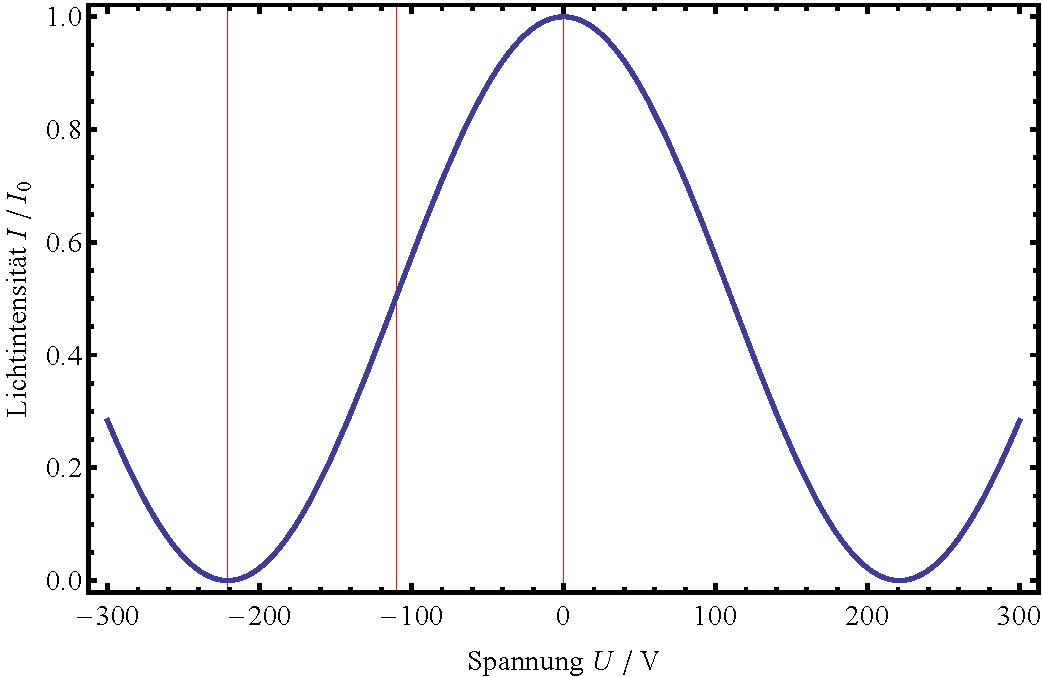
\includegraphics[width=0.8\textwidth]{../img/Pocktheo1.pdf}
  \caption{figureCaption.}
  \label{img:pocktheo1}
\end{center}
\end{figure}

\begin{figure}[H]
\begin{center}
  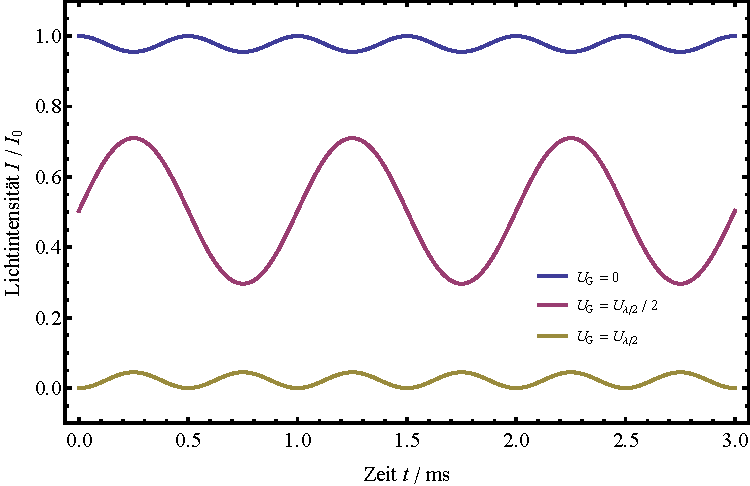
\includegraphics[width=0.8\textwidth]{../img/Pocktheo2.pdf}
  \caption{figureCaption.}
  \label{img:pocktheo2}
\end{center}
\end{figure}

\begin{figure}[H]
\begin{center}
  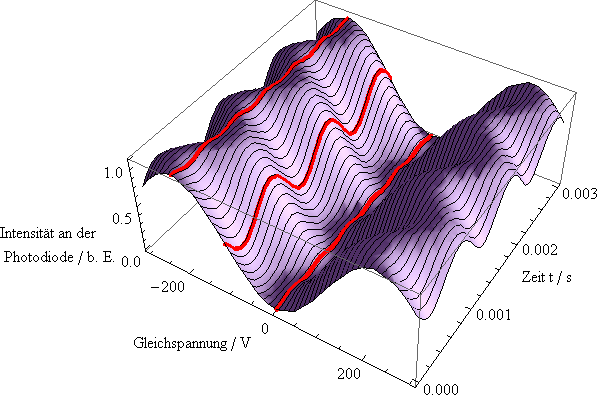
\includegraphics[width=\textwidth]{../img/Pocktheo3.png}
  \caption{figureCaption.}
  \label{img:pocktheo3}
\end{center}
\end{figure}






\begin{figure}[H]
\begin{center}
  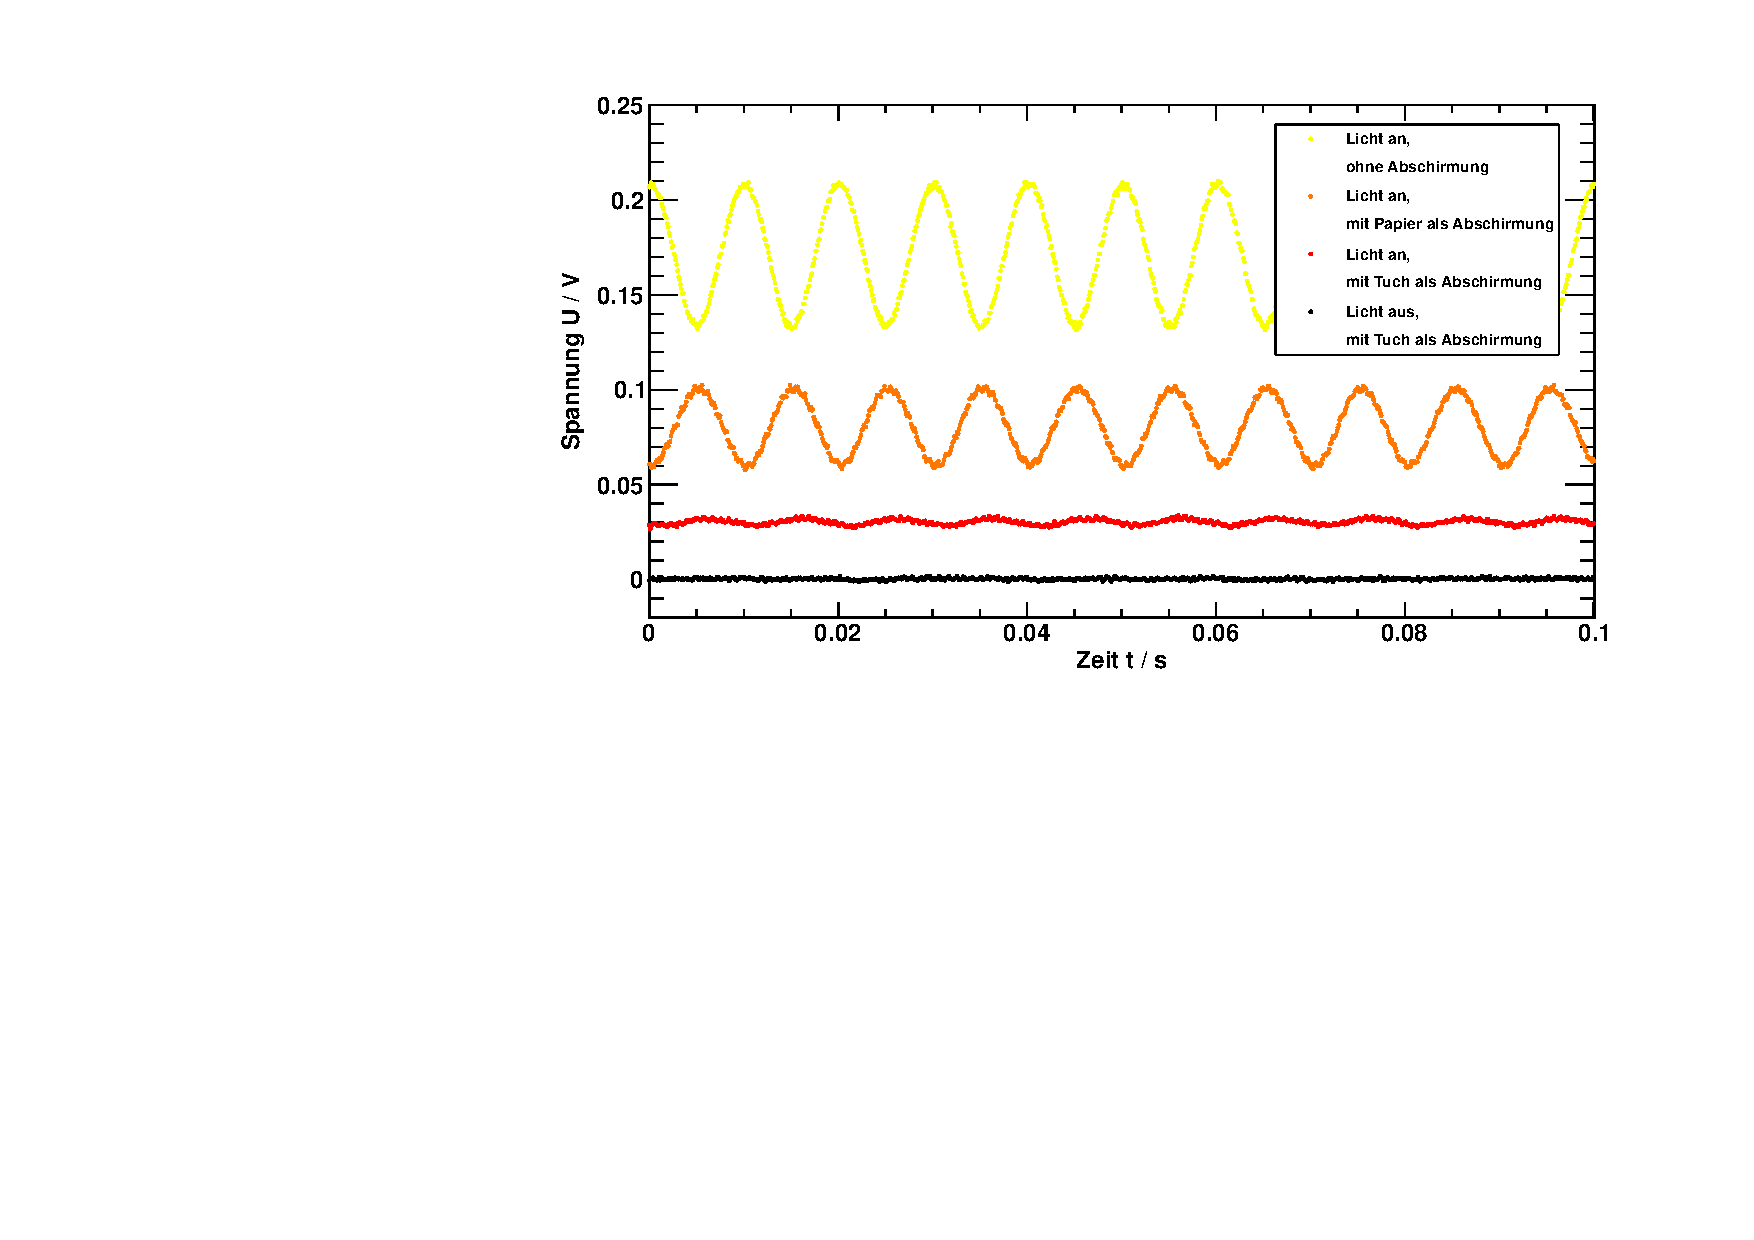
\includegraphics[width=\textwidth]{../img/licht.pdf}
  \caption{Störsignal mit Frequenz 100\,Hz durch die Neonlampen an der Decke des Labors und
  Beseitigung durch geeignete Abschirmung.
  Zur besseren Übersicht wurden die drei oberen Signale mit Offset eingezeichnet. }
  \label{img:licht}
\end{center}
\end{figure}


\subsection{Teil II: Faraday-Effekt}
-erwähne Messreihenfolge --> Aufspüren systematischer Fehler \\
-Bild für verschiedene Einstellungen von Halbschattenpolarimeter